\documentclass[mathserif]{beamer}
\usepackage{amsmath}
\usepackage{url}
\usepackage{tikz}
\beamertemplatenavigationsymbolsempty
\mode<presentation>
\usetheme{Madrid}
\AtBeginSection[]{}
\setbeamerfont{footnote}{size=\tiny}
\title{Phase Transitions in Networks of Memristive Elements}
\author{Forrest Sheldon}
\institute{UCSD}
\date{August 21, 2015}
\titlegraphic{
\includegraphics[width=2.5cm]{gl-1-logo.png}}
\begin{document}

\begin{frame}
\titlepage
\end{frame}

\begin{frame}
\frametitle{A Perspective On Memristors}
\setbeamercovered{static}
\begin{columns}
\column{0.5\textwidth}
\begin{center}
\onslide<1->{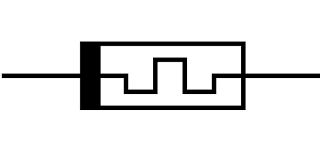
\includegraphics[width=0.17\textwidth]{memristor.png}}

\only<1>{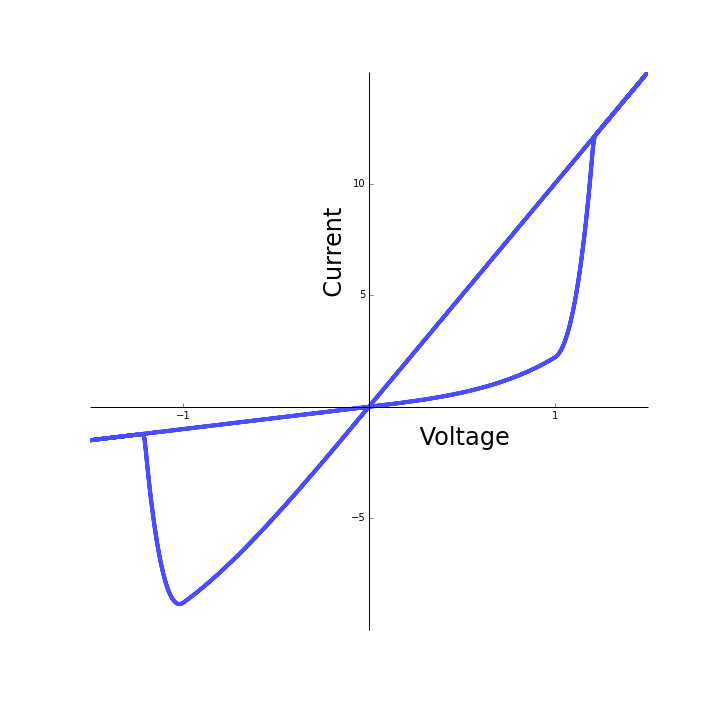
\includegraphics[width=0.65\textwidth]{hysteresis.png}}

\only<2>{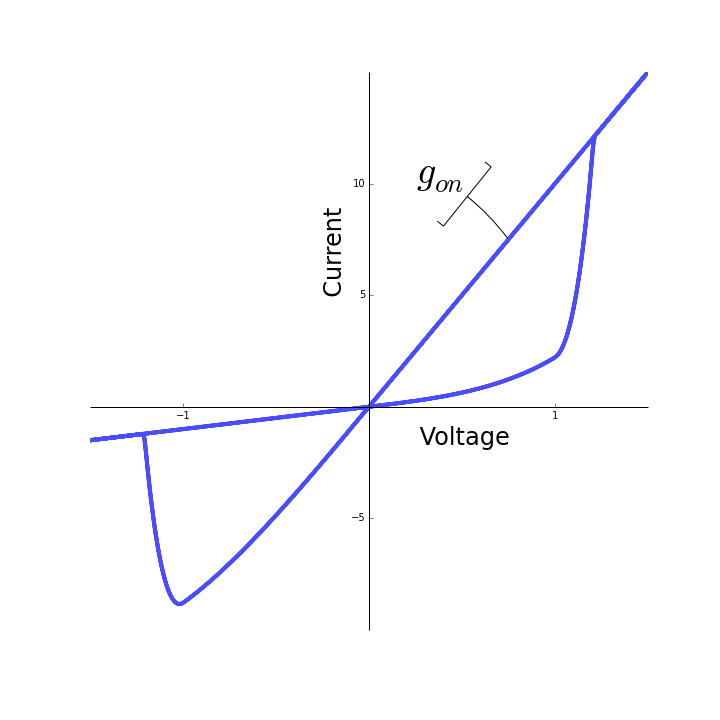
\includegraphics[width=0.65\textwidth]{hysteresis_on.png}}

\only<3>{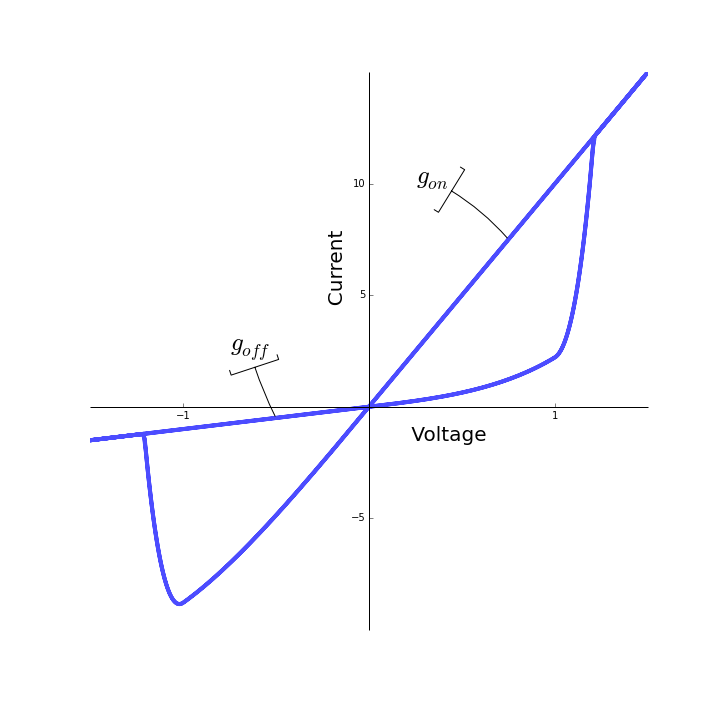
\includegraphics[width=0.65\textwidth]{hysteresis_off.png}}

\onslide<4->{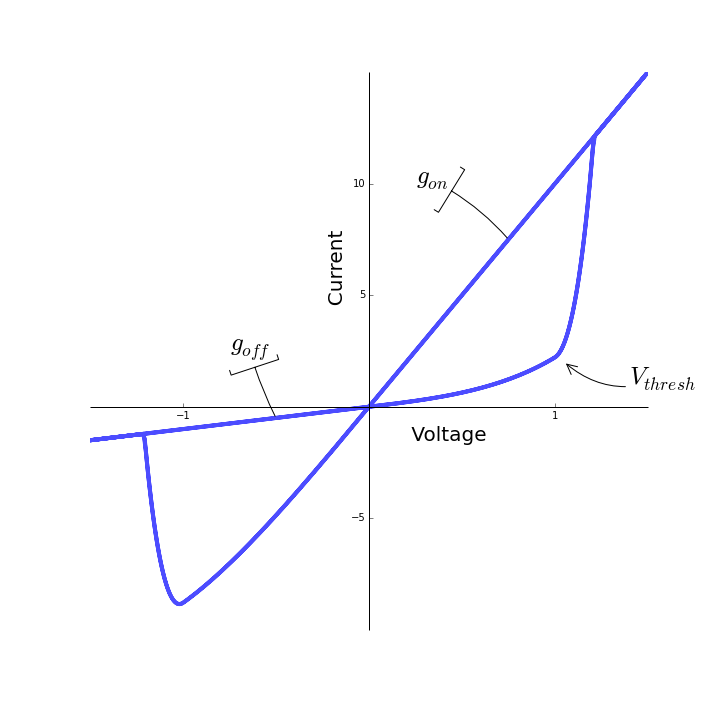
\includegraphics[width=0.65\textwidth]{hysteresis_thresh.png}}

\end{center}
\column{0.5\textwidth}
\centering
\onslide<6->{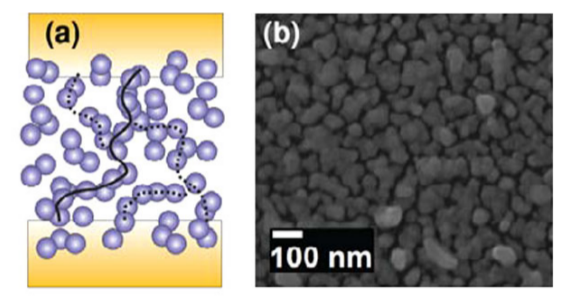
\includegraphics[width=0.65\textwidth]{Granular_short.png}}
\onslide<6->{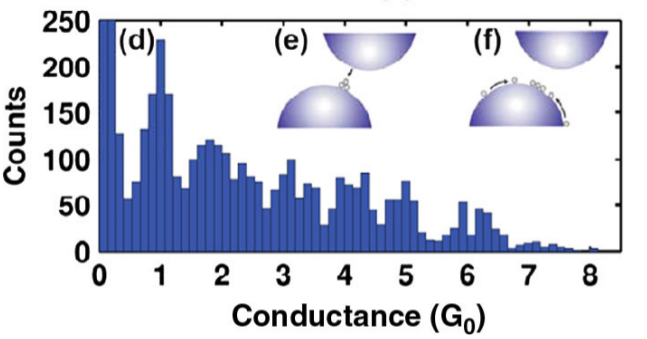
\includegraphics[width=0.65\textwidth]{Granular_low.png}\footnote[frame]{A. Sattar, S.Fostner, and S. Brown, Phys. Rev. Lett. \textbf{111}, 13 (2013).}}
\end{columns}
\begin{center}
\onslide<5->{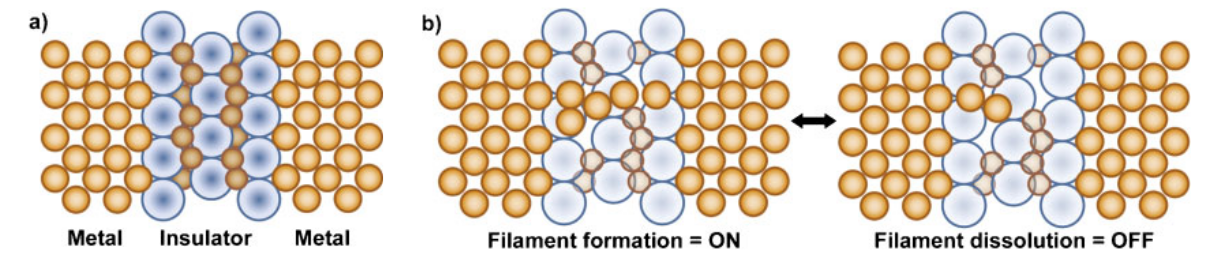
\includegraphics[width=0.8\textwidth]{Atomic_Switch_Filament.png}\footnote[frame]{A. Z. Steig \emph{et al.}, Jpn. J. Appl. Phys. \textbf{53} 01AA02 (2014).}}

\end{center}

\end{frame}

\begin{frame}
\frametitle{'Nonideal' Properties are Interesting}

\begin{center}
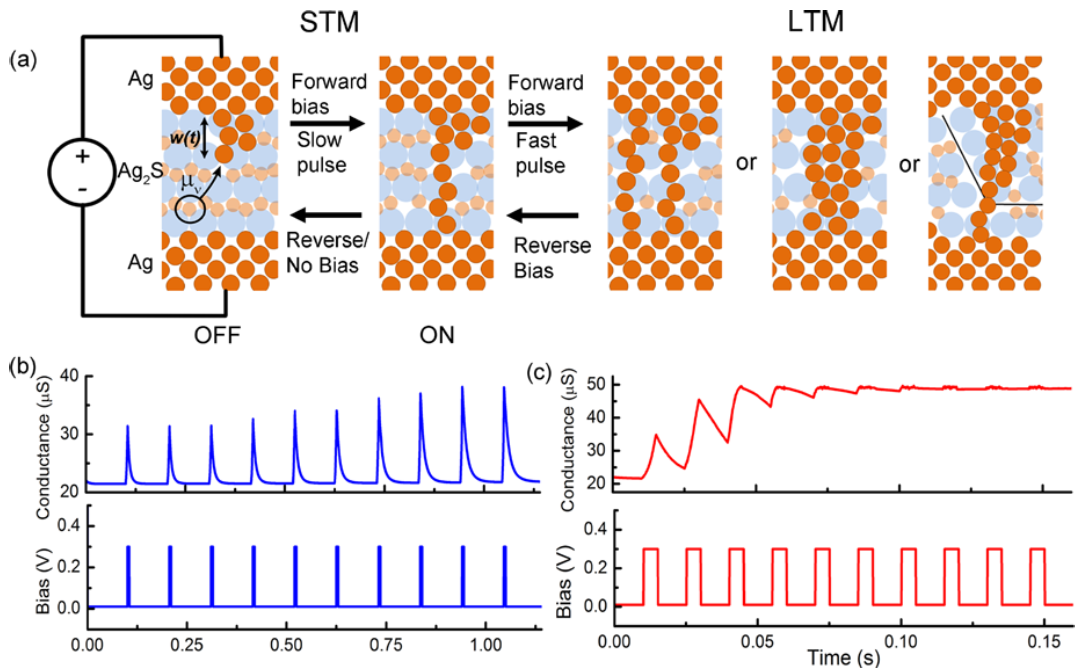
\includegraphics[width=0.8\textwidth]{STM_LTP.png}\footnote{A.Z. Steig \emph{et al.}, in \emph{Memristor Networks}, editted by A. Adamatzky, L. Chua, (Springer International Publishing, 2014)}
\end{center}
\end{frame}

\begin{frame}
\frametitle{Memristive Networks}
\begin{columns}
\column{0.5\textwidth}
\begin{center}
\onslide<1->{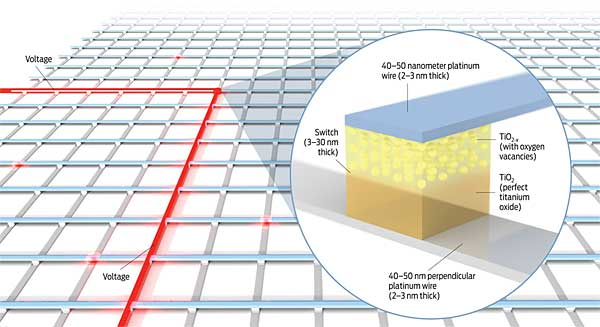
\includegraphics[width=0.7\textwidth]{Crossbar.jpeg}\footnote[frame]{\url{http://spectrum.ieee.org/semiconductors/processors/how-we-found-the-missing-memristor/memrf1}}}
\vspace{0.1in}

\onslide<4->{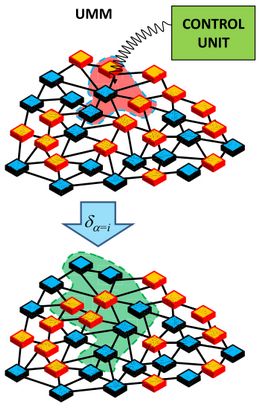
\includegraphics[width=0.4\textwidth]{UMM.png}\footnote[frame]{F. L. Traversa, M. Di Ventra, IEEE T Neural Networks and Learning Systems, \textbf{PP}, 90 (2015).}}

\end{center}
\column{0.5\textwidth}
\begin{center}
\onslide<2->{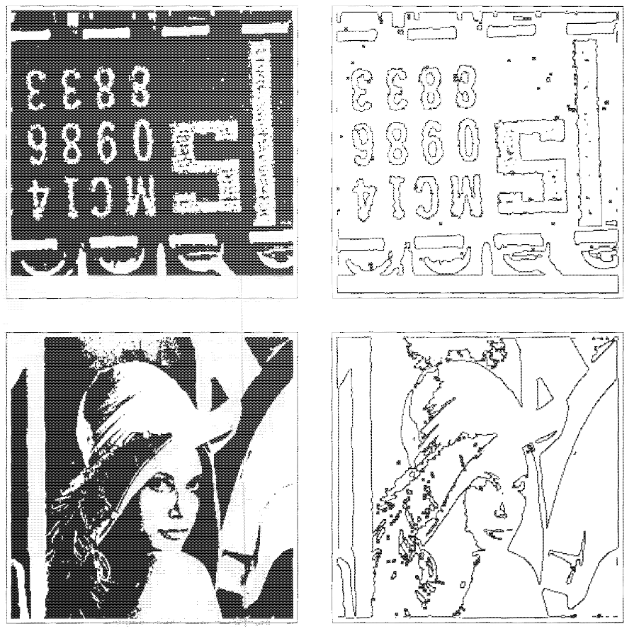
\includegraphics[width=0.6\textwidth]{Cell_Auto_Edge.png}\footnote[frame]{M. Itoh, L. O. Chua, Int.. J. Bifurcat. Chaos, \textbf{19}, 11 (2009).}}
\vspace{0.2in}

\onslide<3->{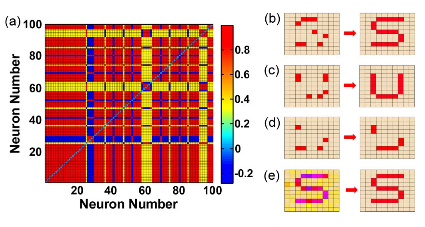
\includegraphics[width=0.6\textwidth]{Associative_Memory.png}\footnote[frame]{D. Kuzum \emph{et al.} IEEE Trans. on Elec. Dev., \textbf{59}, 12 (2012)}}

\end{center}
\end{columns}
\end{frame}

\begin{frame}
\frametitle{Atomic Switch Network}

\begin{center}
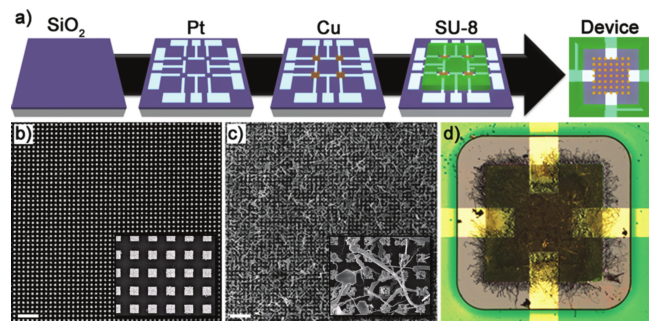
\includegraphics[width=9cm]{ASN_fabrication.png}\footnote{A. Z. Stieg \emph{et al.}, Adv. Mater. \textbf{24}, (2012).}
\end{center}

\begin{columns}
\column{0.5\textwidth}
\centering
\onslide<2->{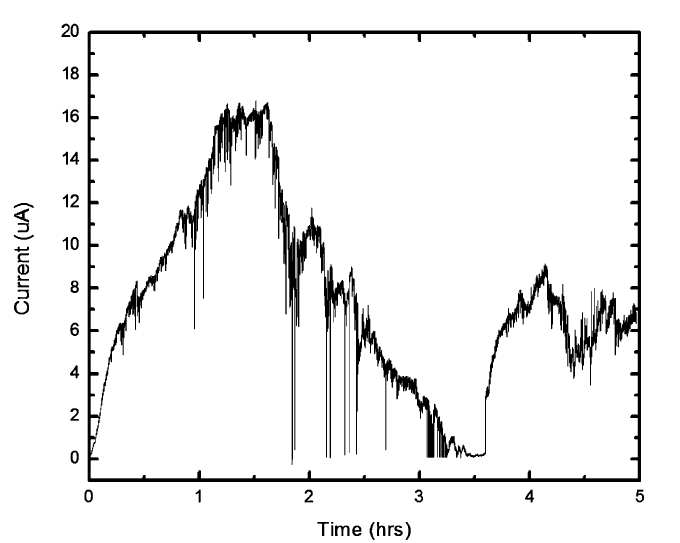
\includegraphics[width=0.5\textwidth]{ASN_fluctuations.png}}
\column{0.5\textwidth}
\centering
\onslide<3->{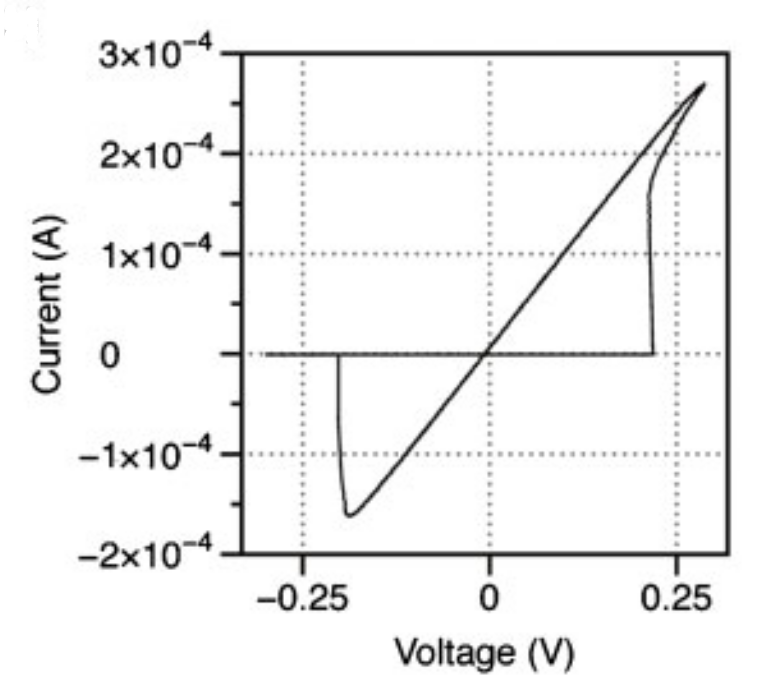
\includegraphics[width=0.5\textwidth]{ASN_hysteresis.png}}
\end{columns}

\end{frame}

\begin{frame}
\frametitle{Questions}
\setbeamercovered{dynamic}
\begin{itemize}
\item<1> Phase Transitions?
\item<2> Role of ON/OFF ratio and disorder?
\item<3> Avalanches?
\end{itemize}
\end{frame}

\begin{frame}
\frametitle{Modeling the Network}
\begin{picture}(320, 250)
\onslide<1->{\put(0, 210){Timescales}}
\onslide<1->{\put(110, 174){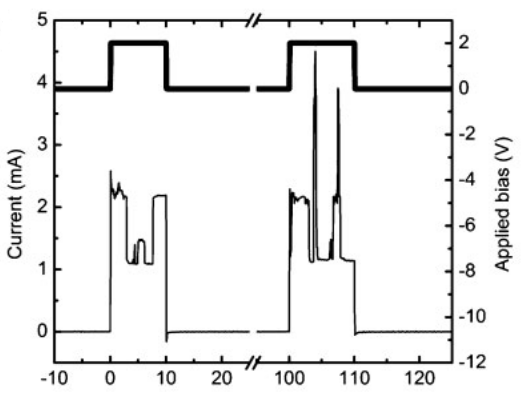
\includegraphics[width=1.25in]{ASN_jumps.png}}}
\onslide<2->{\put(220, 164){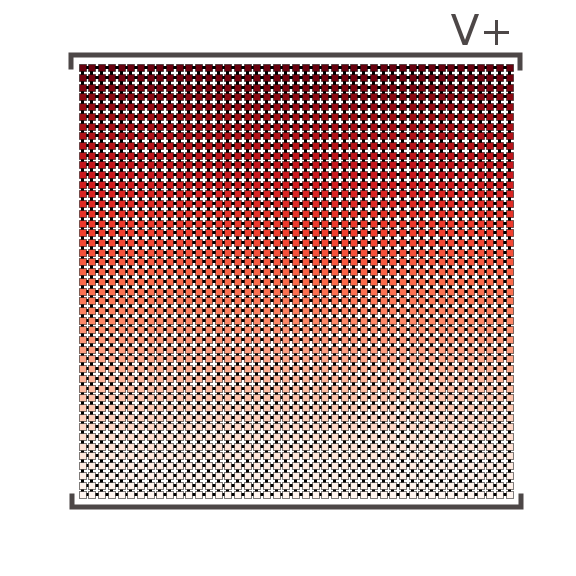
\includegraphics[width=1.2in]{harmonic_voltage_brackets.png}}}

\onslide<3->{\put(0, 160){Thresholds}}

\onslide<4->{\put(0, 110){Network Structure}}
\onslide<4->{\put(120, 103){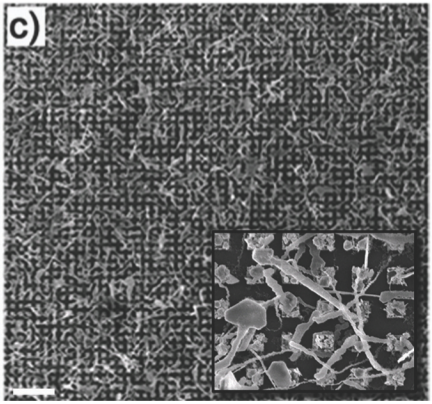
\includegraphics[width=0.95in]{ASN_structure.png}}}
\onslide<5->{\put(220, 91){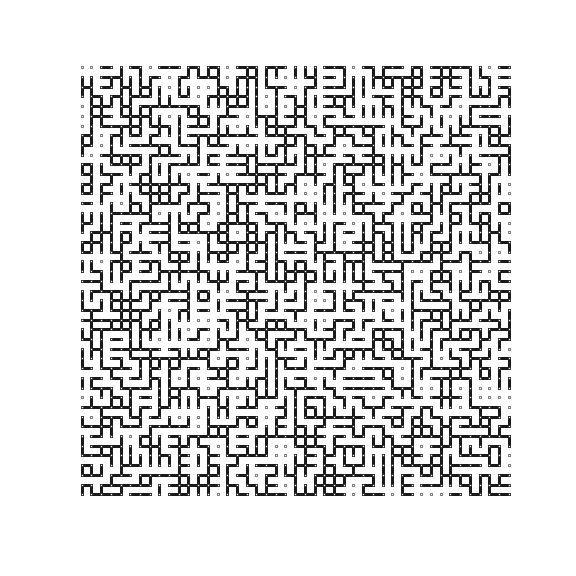
\includegraphics[width=1.2in]{RR_cond.png}}}

\onslide<6->{\put(0, 60){Disordered$\to$Regular}}
\onslide<6->{\put(110, 13){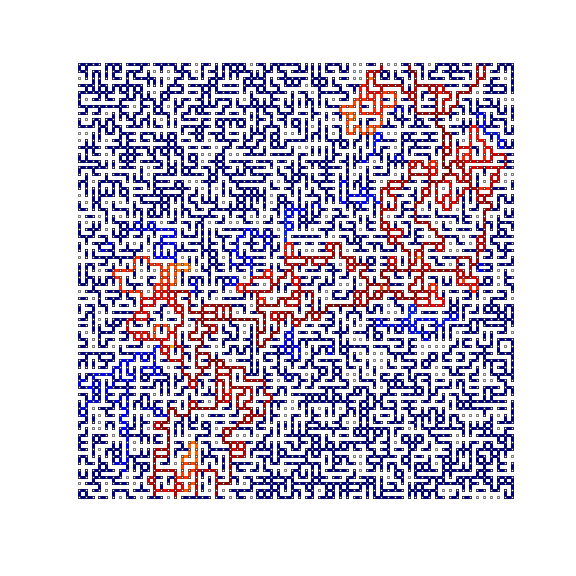
\includegraphics[width=1.2in]{RR_logvoltage.png}}}
\onslide<7->{\put(217, 10){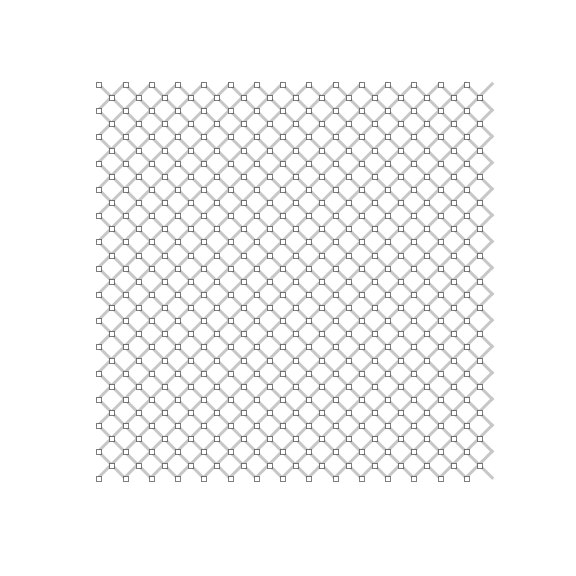
\includegraphics[width=1.3in]{diag_network.png}}}

\end{picture}
\end{frame}

\begin{frame}
\frametitle{Our Model}
\begin{columns}
\column{0.5\textwidth}
\begin{center}
\onslide<1->{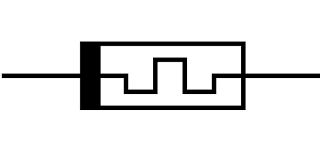
\includegraphics[width=0.25\textwidth]{memristor.png}}

\only<1>{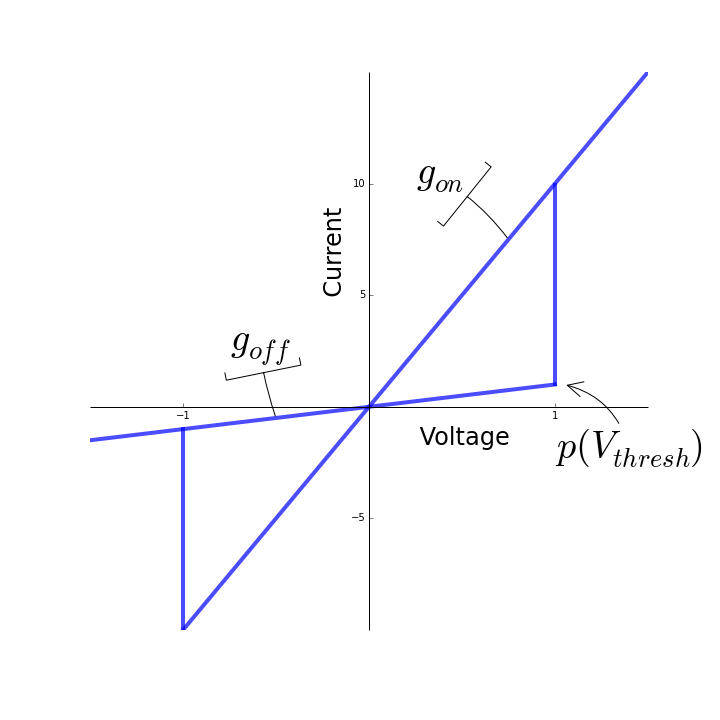
\includegraphics[width=\textwidth]{memristor_model.png}}
\onslide<2->{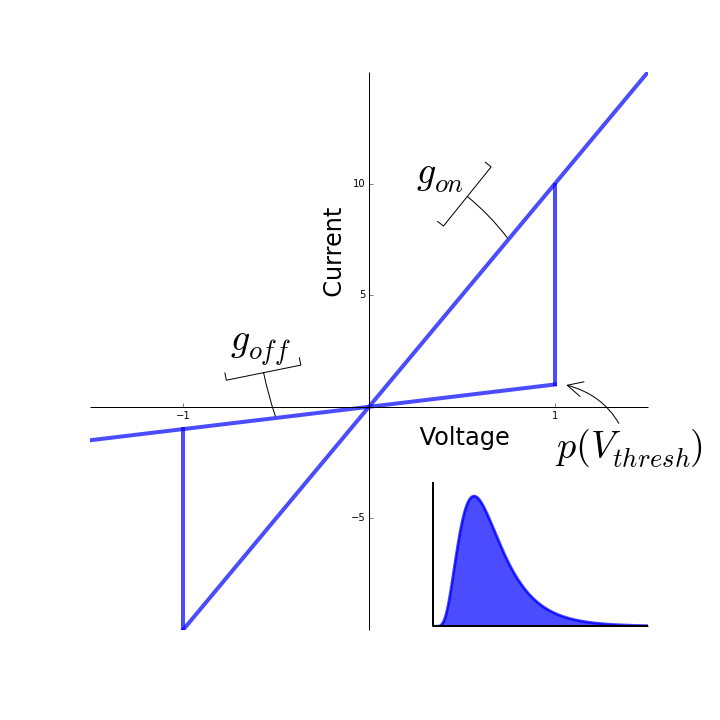
\includegraphics[width=\textwidth]{memristor_model_dist.png}}
\end{center}
\column{0.5\textwidth}
\centering
\onslide<3->{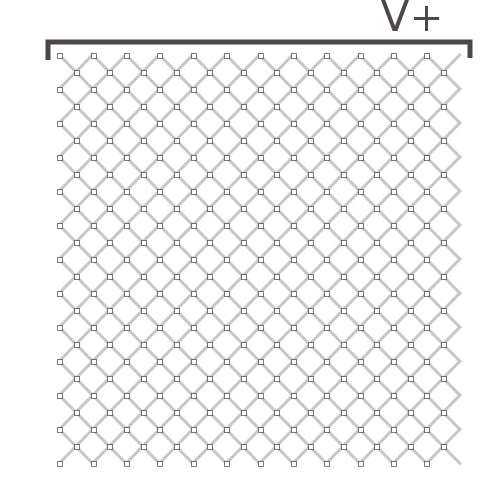
\includegraphics[width=0.4\textwidth]{Inside_a_network_1.png}}

\onslide<4->{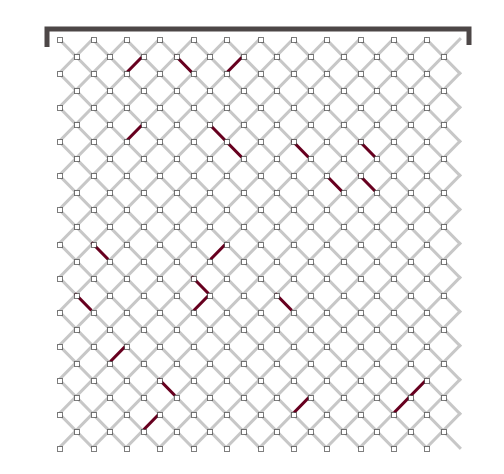
\includegraphics[width=0.4\textwidth]{Inside_a_network_2.png}}

\onslide<5->{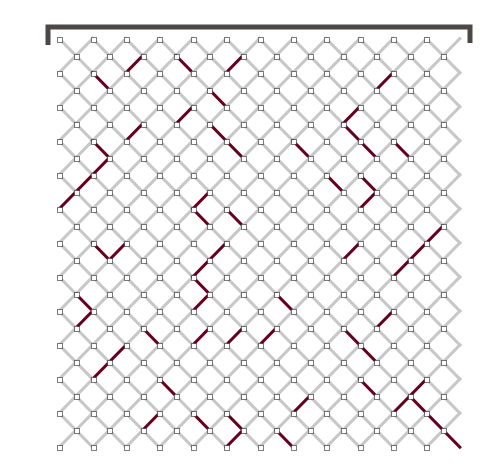
\includegraphics[width=0.4\textwidth]{Inside_a_network_3.png}}

\end{columns}
\end{frame}

\begin{frame}
\frametitle{Simulating Memristor Networks}
\begin{center}

\only<1>{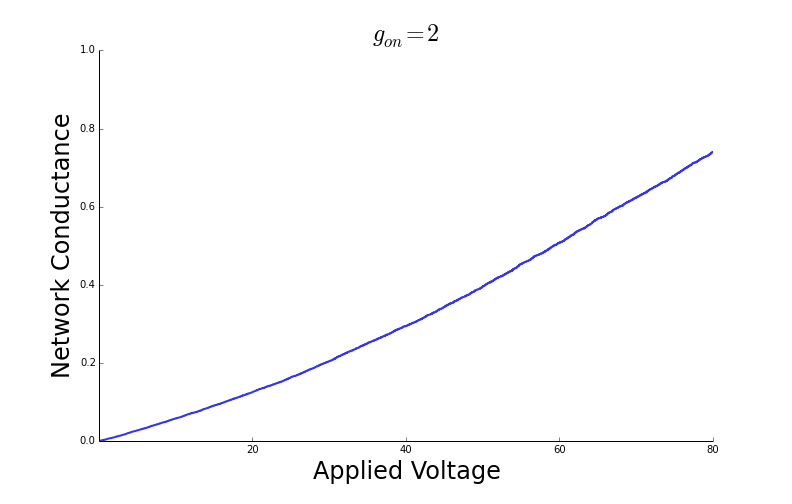
\includegraphics[width=\textwidth]{2DL45ON2_cond.png}}

\only<2>{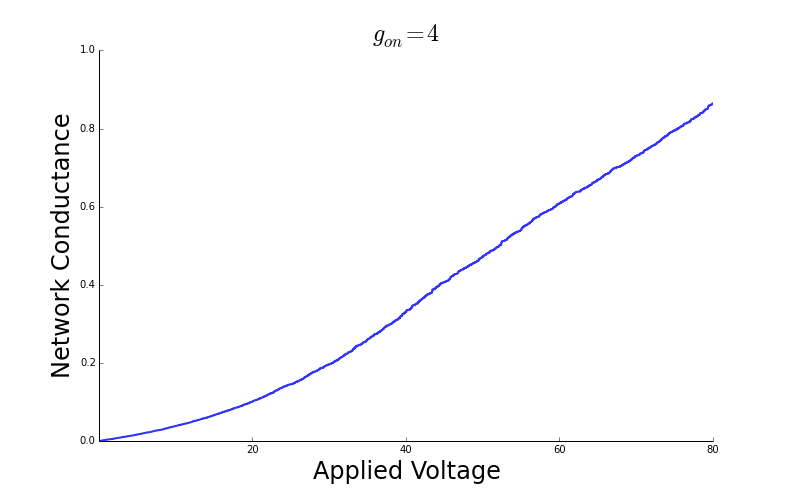
\includegraphics[width=\textwidth]{2DL45ON4_cond.png}}

\only<3>{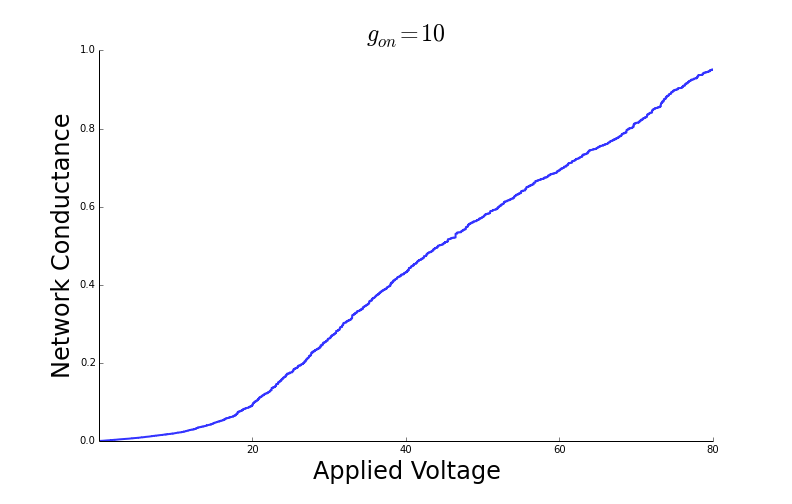
\includegraphics[width=\textwidth]{2DL45ON10_cond.png}}

\only<4>{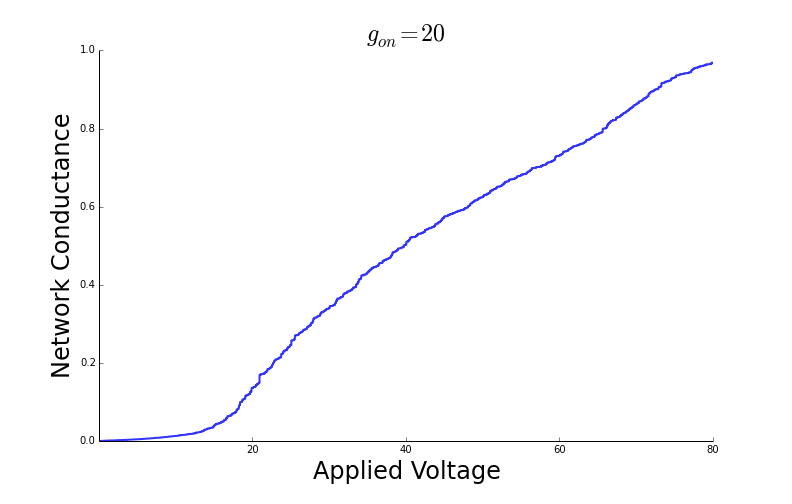
\includegraphics[width=\textwidth]{2DL45ON20_cond.png}}

\only<5>{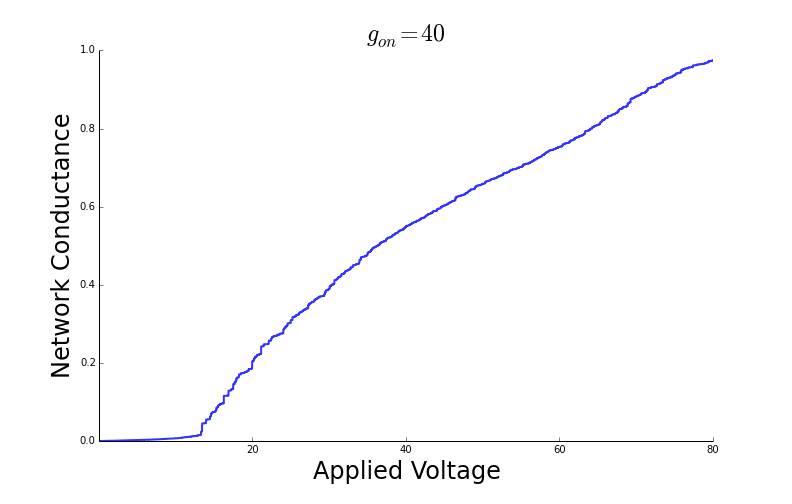
\includegraphics[width=\textwidth]{2DL45ON40_cond.png}}

\only<6>{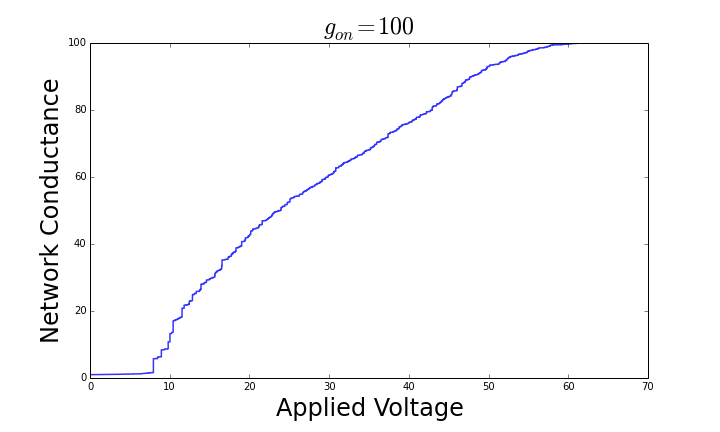
\includegraphics[width=\textwidth]{2DL45ON100_cond.png}}

\only<7>{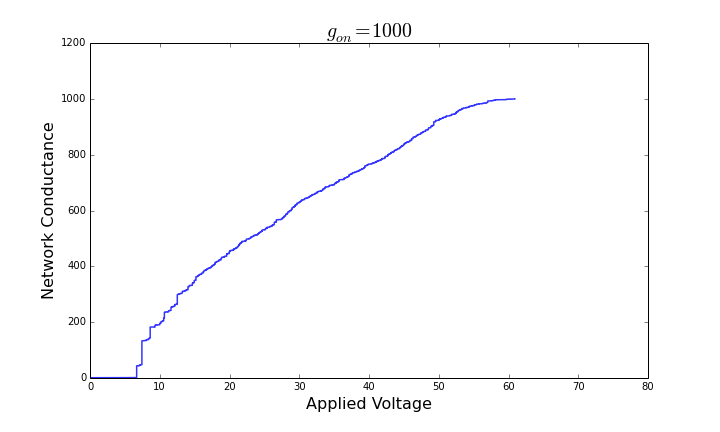
\includegraphics[width=\textwidth]{2DL45ON1000_cond.png}}

\end{center}
\end{frame}

\begin{frame}
\frametitle{Internal Dynamics}

\end{frame}

\begin{frame}
\frametitle{Mean-Field Theory\footnote[frame]{S. Zapperi \emph{et al.} Phys. Rev. E \textbf{59}, 5049 (1999).}}

\onslide<1->{$$P = \sum_i \sigma_i \Delta V_i^2$$}

\onslide<2->{$$P = G(\{\sigma_i\})V^2$$}

\onslide<3->{Effective Medium Theory, $G(\{\sigma_i\}) \approx G(f), \quad f = \frac{n_{on}}{N}$}

\onslide<4->{$$\phi = \frac{\sum_i \sigma_i}{N} = g_{off} + f(g_{on} - g_{off})\quad G(f) \to G(\phi)$$}

\onslide<5->{$$P = \sum_i \sigma_i \frac{G(\phi)V^2}{\phi N}$$}

\end{frame}


\begin{frame}
\frametitle{Self-Consistency Equation}

\onslide<1->{$$\Delta V_{MF} = \sqrt{\frac{G(\phi)}{\phi}}\frac{V}{\sqrt{N}} = h(\phi)v$$}
\onslide<2->{Average across network realizations,
$$\langle\phi\rangle = g_{off} P(t>h(\phi)v) + g_{on} P(t< h(\phi)v)$$
}
\only<3>{
$$\phi = g_{off} + (g_{on}-g_{off}) \int_0^{h(\phi)v} p(t) dt$$
}
\only<4->{
$$f = \int_0^{h(f)v} p(t) dt$$
}
\onslide<3->{
\centering
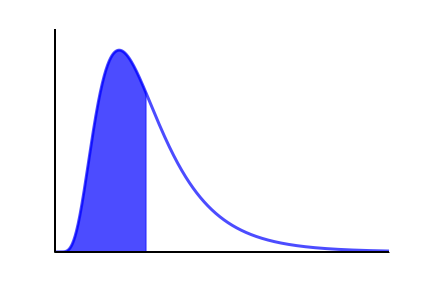
\includegraphics[width=0.4\textwidth]{dist_init.png}
}



\end{frame}

\begin{frame}
\frametitle{One-Dimensional Networks}
\centering
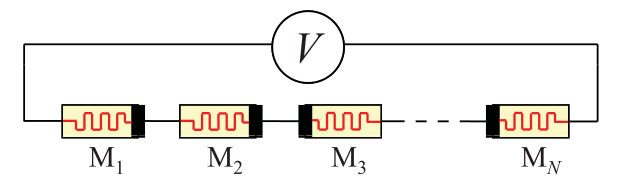
\includegraphics[width=0.4\textwidth]{1D_memristor_chain.png}

\begin{columns}
\column{0.5\textwidth}
$$G(f)V = \frac{g_{on}g_{off}}{(g_{on} - f (g_{on} - g_{off}))}\frac{V}{N}$$
\centering
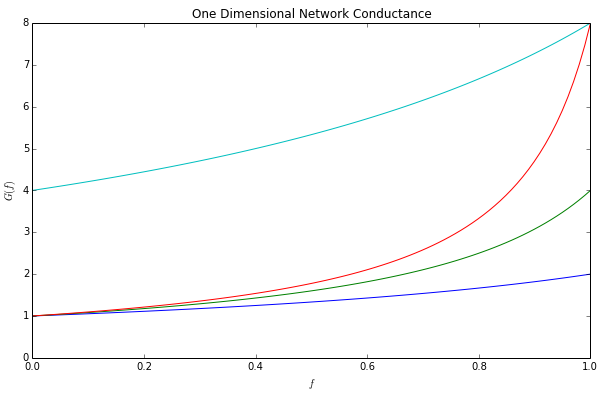
\includegraphics[width=\textwidth]{1D_Network_Cond.png}

\column{0.5\textwidth}
\onslide<2->{$$f = \int_0^{G(f)V} p(t) dt$$}
\begin{center}

\only<2>{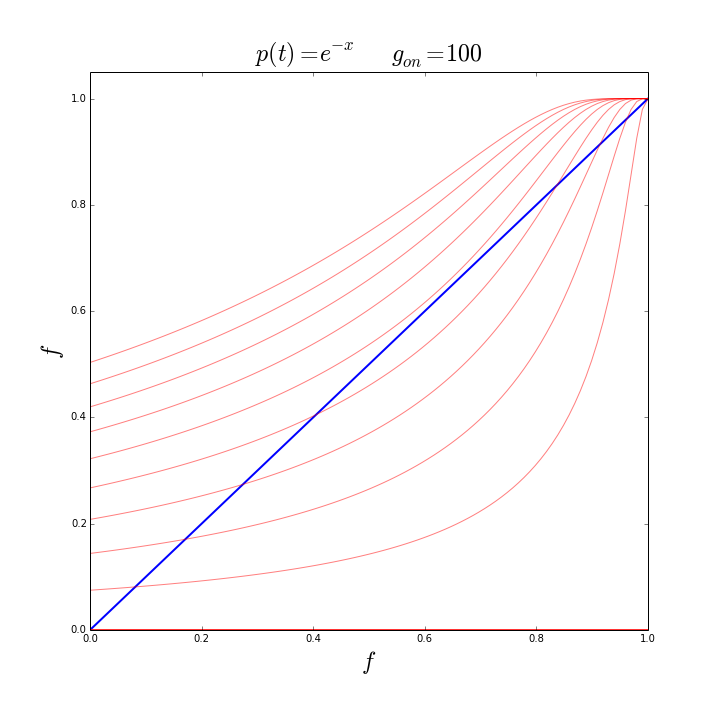
\includegraphics[width=0.8\textwidth]{SC_1D_ON100_expon_0.png}}

\only<3>{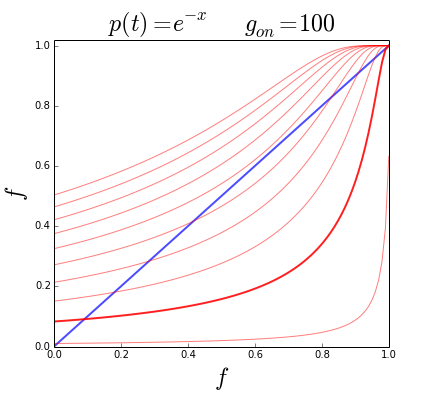
\includegraphics[width=0.8\textwidth]{SC_1D_ON100_expon_1.png}}

\only<4>{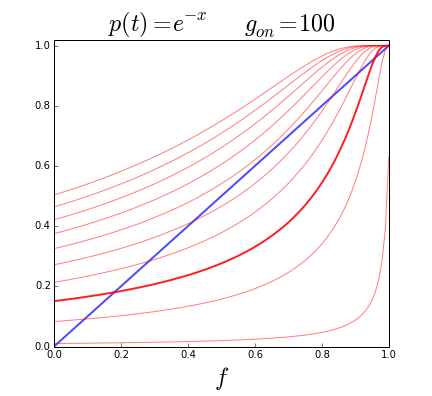
\includegraphics[width=0.8\textwidth]{SC_1D_ON100_expon_2.png}}

\only<5>{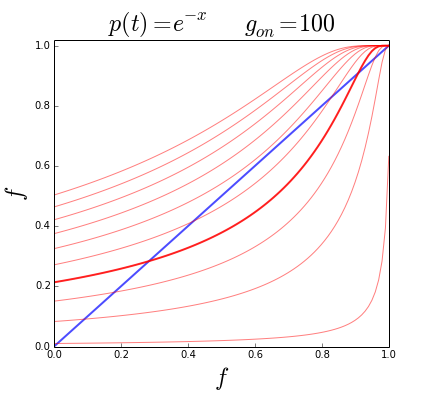
\includegraphics[width=0.8\textwidth]{SC_1D_ON100_expon_3.png}}

\only<6>{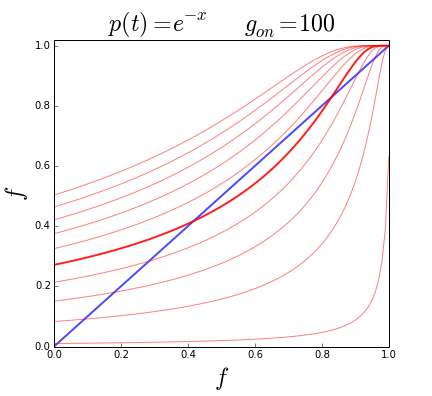
\includegraphics[width=0.8\textwidth]{SC_1D_ON100_expon_4.png}}

\only<7>{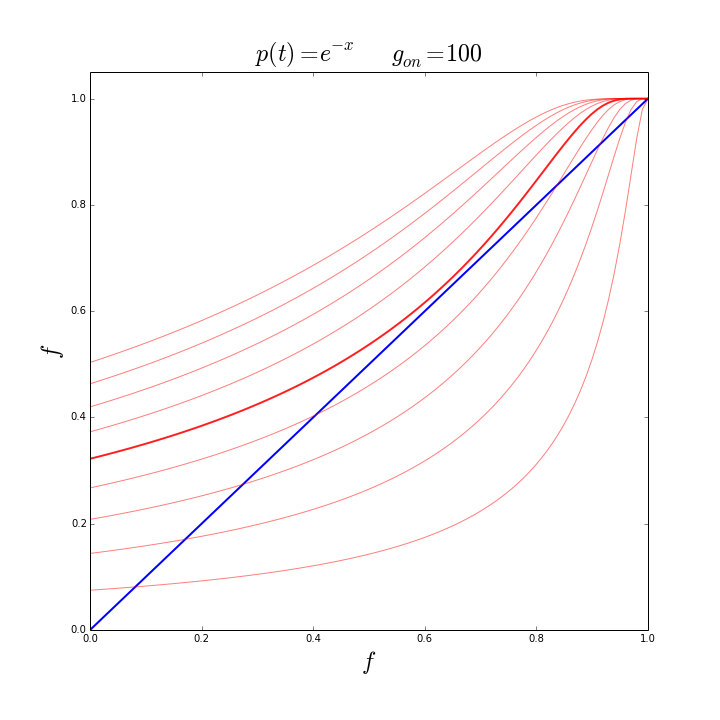
\includegraphics[width=0.8\textwidth]{SC_1D_ON100_expon_5.png}}

\only<8>{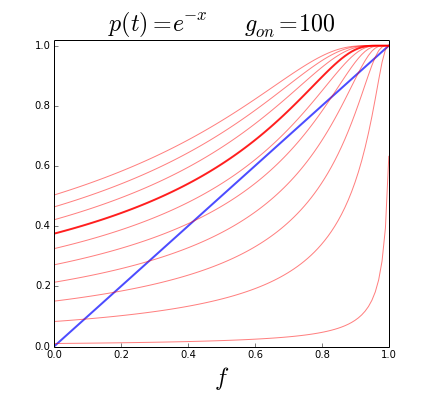
\includegraphics[width=0.8\textwidth]{SC_1D_ON100_expon_6.png}}

\only<9>{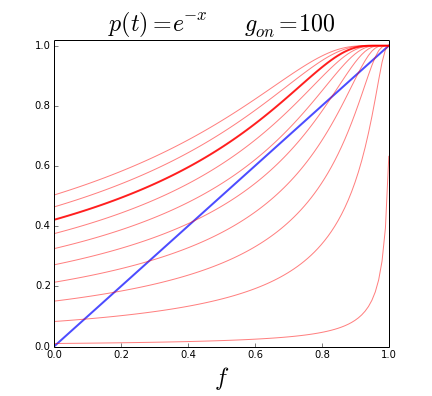
\includegraphics[width=0.8\textwidth]{SC_1D_ON100_expon_7.png}}

\only<10>{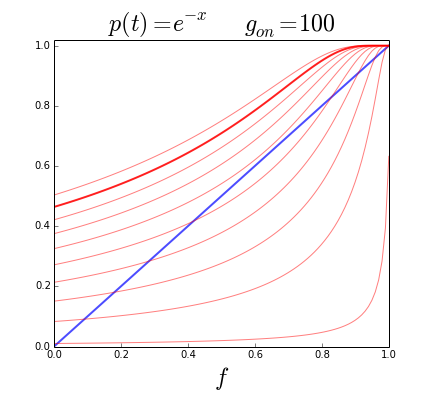
\includegraphics[width=0.8\textwidth]{SC_1D_ON100_expon_8.png}}

\only<11>{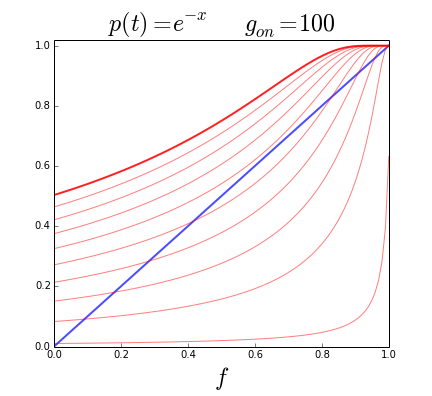
\includegraphics[width=0.8\textwidth]{SC_1D_ON100_expon_9.png}}

\end{center}

\end{columns}
\end{frame}

\begin{frame}
\frametitle{Reduction to the ON/OFF Ratio}
\onslide<1->{$$G(f)V = \frac{g_{on}g_{off}}{(g_{on} - f (g_{on} - g_{off}))}\frac{V}{N}\to \frac{1}{1 - f(1-\alpha)}\frac{g_{off}V}{N}\quad\alpha = \frac{g_{off}}{g_{on}}$$}
\begin{center}

\only<1>{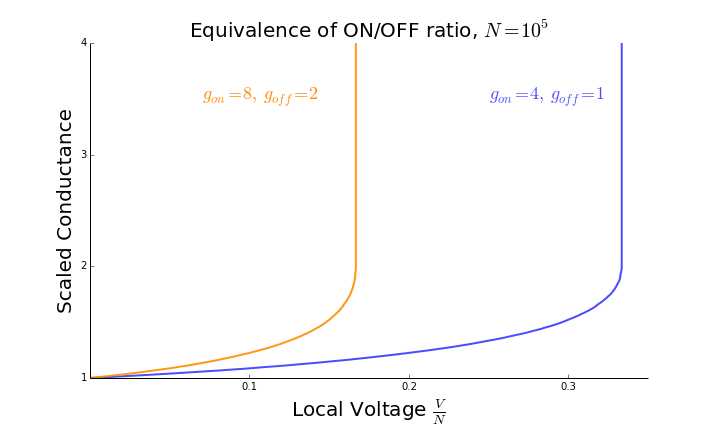
\includegraphics[width=0.8\textwidth]{ONOFF_ratio_1.png}}

\onslide<2->{\includegraphics[width=0.8\textwidth]{ONOFF_ratio_2.png}}

\end{center}
\end{frame}


\begin{frame}
\frametitle{Finding the transition}
First order phase transition:
$$f = \int_0^{G(f)V} p(t) dt,  \quad\quad 1 = p(G(f)V)G'(f)V \quad 0 \le f \le 1$$
For Uniform(0,T),
$f_c = \frac{1}{2(1-\alpha)}, \: V_c = \frac{TN}{4g_{off}(1-\alpha)},
 \: \alpha = \frac{g_{off}}{g_{on}}$

\vspace{0.25in}
\centering
\includegraphics[width=1.1\textwidth]{SC_1D_Uniform01.png}

\end{frame}

\begin{frame}
\frametitle{Finding the Transition}
\centering
$f_c = \frac{1}{2(1-\alpha)}, \: V_c = \frac{TN}{4g_{off}(1-\alpha)},
 \: \alpha = \frac{g_{off}}{g_{on}}$
\includegraphics[width=0.8\textwidth]{1D_Cond.png}

\end{frame}

\begin{frame}
\frametitle{Two-Dimensional Networks}
\begin{center}
\onslide<1->{$$\Delta V_{MF} = \sqrt{\frac{G(f)}{\phi(f)}}\frac{V}{\sqrt{N}} = h(f)v$$}
\onslide<2->{$$G(f) = \frac{(2f-1)(g_{on}-g_{off}) + \sqrt{(2f-1)^2(g_{on}-g_{off})^2 + 4g_{on}g_{off}}}{2}$$}
\onslide<3->{\includegraphics[width=0.8\textwidth]{MF_upper_limit.png}}
\end{center}

\end{frame}


\begin{frame}
\frametitle{ON/OFF ratio Induced Transition}
$p(t) = e^{-t}$
\begin{center}

\includegraphics[width=\textwidth]{SC_2D_Exponential_set.png}
\end{center}
\end{frame}

\begin{frame}
\frametitle{Avalanches}
\only<1>{\begin{center}
\includegraphics[width=0.4\textwidth]{dist_init.png}

Switching a memristor: $f\to f+\frac{1}{N}$
\end{center}
}
\only<2>{\begin{center}
\includegraphics[width=0.4\textwidth]{dist_first_switch.png}

Changes the current, $h(f)V\to h(f)V + \frac{h'(f)V}{N}$
\end{center}
}
\only<3>{\begin{center}
\includegraphics[width=0.4\textwidth]{dist_first_switch.png}
$$P(n) \to \frac{(\mu)^n}{n!} e^{-\mu}, \quad \mu = p(h(f)v)h'(f)v$$
\end{center}
}
\only<4>{\begin{center}
\includegraphics[width=0.4\textwidth]{dist_2nd_switch.png}
$$P(n) \to \frac{(\mu)^n}{n!} e^{-\mu}, \quad \mu = p(h(f)v)h'(f)v$$
\end{center}
}
\only<5>{\begin{center}
\includegraphics[width=0.4\textwidth]{dist_2nd_switch_separate.png}
$$P(n) \to \frac{(\mu)^n}{n!} e^{-\mu}, \quad \mu = p(h(f)v)h'(f)v$$
\end{center}
}
\only<6>{\begin{center}
\includegraphics[width=0.4\textwidth]{dist_N2inf.png}
$$P(n) \to \frac{(\mu)^n}{n!} e^{-\mu}, \quad \mu = p(h(f)v)h'(f)v$$
\end{center}
}

\end{frame}


\begin{frame}
\frametitle{Branching Process with Poissonian Offspring}

\begin{center}
\only<1>{$$P(n) \to \frac{(\mu)^n}{n!} e^{-\mu}, \quad \mu = p(h(f)v)h'(f)v$$
\includegraphics[width=0.4\textwidth]{branch.png}}

\only<2>{\includegraphics[width=\textwidth]{Avalanche_fullrun.png}}

\only<3>{\includegraphics[width=\textwidth]{Avalanche_beginrun.png}}

\only<4>{\includegraphics[width=\textwidth]{Diffusive.png}}

\only<5>{\includegraphics[width=\textwidth]{SubCritical.png}}

\only<6>{\includegraphics[width=\textwidth]{SuperCrit.png}}

\end{center}

\end{frame}


\begin{frame}
\frametitle{Avalanche Size Distribution}
\onslide<1->{
\centering
\includegraphics[width=0.25\textwidth]{branch_Z.png}}
\onslide<2->{$$S = \lim_{n\to\infty} Y_n = 1 + Z_1 + Z_2 + ...+Z_n$$}
\onslide<4->{$$\rho(z) = \sum_{s=1}^\infty z^s \frac{(\mu s)^{s-1}}{s!} e^{-\mu s}$$}

\end{frame}

\begin{frame}
\frametitle{Avalanche Size Distribution}
Borel Distribution, $P(s) = \frac{(\mu s)^{s-1}}{s!} e^{-\mu s}$ $s=1, 2, 3...$
$$E(S) = \frac{1}{1-\mu}$$
$$Var(S)=\frac{\mu}{(1-\mu)^3}$$

\end{frame}

\begin{frame}
\frametitle{Avalanches on Randomly Dilute Lattice $p=0.6$}
\onslide<1->{As $\mu\to 1$ we approach a critical branching process
$$P(s) \sim s^{-3/2}$$}
\onslide<2->{
\centering
\includegraphics[width=0.9\textwidth]{Avalanche_Lattice.png}
}

\end{frame}

\begin{frame}
\frametitle{Future Work}
\begin{columns}
\column{0.5\textwidth}
\onslide<1->{\includegraphics[width=0.9\textwidth]{Current_MF.png}}
\begin{itemize}
\item<1-> Phase Transitions in Current Controlled Networks
\item<2-> Pattern Formation
\item<3-> Including Thermal Effects
\end{itemize}
\column{0.5\textwidth}
\begin{center}

\onslide<2->{\includegraphics[width=0.6\textwidth]{Cell_Aut_Serp.png}}

\onslide<3->{\includegraphics[width=\textwidth]{ASN_Fluct.png}}

\end{center}
\end{columns}
\end{frame}

\begin{frame}
\frametitle{Superconducting Memristors\footnote[frame]{S. Peotta, M. Di Ventra, Phys. Rev. Applied \textbf{2}, 034011 (2014).}}

\onslide<1->{Low Frequency Josephson Junction
$$I = C\frac{dV}{dt} + G_L(1 + \epsilon \cos \gamma)V + I_c \sin \gamma + I_F (t)$$}
\onslide<2->{
\begin{center}
Isolate with CA SQUID\\
\includegraphics[width=0.25\textwidth]{CASQUID.png}
$$I = G'_L (1 + \epsilon' \cos \gamma)V\quad \frac{d\gamma}{dt} = \frac{2e}{\hbar}V$$}
\end{center}
\end{frame}

\begin{frame}
\frametitle{Fluctuation Dissipation Relations for Memristive Elements}
\onslide<1->{Noise Autocorrelation Function
$$\langle I_F (t) I_F (t')\rangle = 2k_B TG'_L [1 + \epsilon ' \cos \gamma(t')]\delta(t - t')$$}
\begin{itemize}
\item<1->{General Memristive Form?}
\item<2->{Link to Hydrodynamics and Spatial Correlations?}


\end{itemize}

\end{frame}

\end{document}
